
% ---------------------- % INSTRUCTIONS % ---------------------- %
% Compile this and save the PDF
% This PDF can then be uploaded as a figure to the repository and included in main.tex

\documentclass[tikz]{standalone}
\usepackage{tikz}
\usetikzlibrary{shapes.geometric}
\usetikzlibrary{arrows.meta}

% Nice captions.
\usepackage[hang,small,bf]{caption}
\setlength{\captionmargin}{25pt}

% Unfortunately we have to do some more in-depth tikz as simple tikz doesn't seem to allow several things

\begin{document}

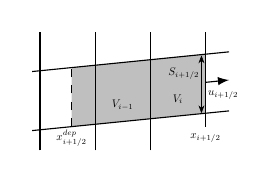
\begin{tikzpicture}[
      scale=0.5,
      solid_line/.style={thick},
      dashed_line/.style={thin,dashed},
      thin_line/.style={thin},
      white_line/.style={thin,white}
    ]

    % ------------------------------------------------------------------ %
    % Draw white box
    % ------------------------------------------------------------------ %

    \draw[white_line] (-0.1cm,-0.1cm) -- (5.5cm,-0.1cm) -- (5.5cm,3.1cm) -- (-0.1cm,3.1cm) -- cycle;


    % ------------------------------------------------------------------ %
    % Draw the element
    % ------------------------------------------------------------------ %

    % swept volume
    \draw[fill=gray, fill opacity=0.5, draw=none] (1.0cm,0.6cm) -- (1.0cm,2.1cm) -- (4.4cm,2.45cm) -- (4.4cm,0.95cm) -- cycle ;
    \draw[dashed_line] (1.0cm,0.6cm) -- (1.0cm,2.1cm) ;

    % x-coordinate lines
    \draw[thin_line] (0cm,0.5cm) -- (5.0cm,1.0cm) ;
    \draw[thin_line] (0cm,2.0cm) -- (5.0cm,2.5cm) ;

    % y-coordinate lines
    \draw[thin_line] (0.2cm,0.0cm) -- (0.2cm,3.0cm) ;
    \draw[thin_line] (1.6cm,0.0cm) -- (1.6cm,3.0cm) ;
    \draw[thin_line] (3.0cm,0.0cm) -- (3.0cm,3.0cm) ;
    \draw[thin_line] (4.4cm,0.6cm) -- (4.4cm,3.0cm) ;

    % arrow for flux
    \draw [-latex](4.4cm,1.725cm) -- (5.0cm,1.785cm);

    % arrow for facet size
    \draw [{Stealth[length=0.1cm]}-{Stealth[length=0.1cm]}, line width=0.2](4.3cm,2.41cm) -- (4.3cm,0.94cm);

    % ------------------------------------------------------------------ %
    % Annotations
    % ------------------------------------------------------------------ %
    \node[anchor=center,scale=0.4] at (4.85cm,1.4cm) {$u_{i+1/2}$} ;
    \node[anchor=center,scale=0.4] at (4.4cm,0.3cm) {$x_{i+1/2}$} ;
    \node[anchor=center,scale=0.4] at (1.0cm,0.3cm) {$x^{dep}_{i+1/2}$} ;
    \node[anchor=center,scale=0.4] at (2.3cm,1.15cm) {$V_{i-1}$} ;
    \node[anchor=center,scale=0.4] at (3.7cm,1.3cm) {$V_i$} ;
    \node[anchor=center,scale=0.4] at (3.85cm,1.95cm) {$S_{i+1/2}$} ;

    \end{tikzpicture}

\end{document} 
